%%% Hlavní soubor. Zde se definují základní parametry a odkazuje se na ostatní části. %%%

%% Verze pro jednostranný tisk:
% Okraje: levý 40mm, pravý 25mm, horní a dolní 25mm
% (ale pozor, LaTeX si sám přidává 1in)
\documentclass[12pt,a4paper]{report}
\setlength\textwidth{145mm}
\setlength\textheight{247mm}
\setlength\oddsidemargin{15mm}
\setlength\evensidemargin{15mm}
\setlength\topmargin{0mm}
\setlength\headsep{0mm}
\setlength\headheight{0mm}
% \openright zařídí, aby následující text začínal na pravé straně knihy
\let\openright=\clearpage

%% Pokud tiskneme oboustranně:
% \documentclass[12pt,a4paper,twoside,openright]{report}
% \setlength\textwidth{145mm}
% \setlength\textheight{247mm}
% \setlength\oddsidemargin{15mm}
% \setlength\evensidemargin{0mm}
% \setlength\topmargin{0mm}
% \setlength\headsep{0mm}
% \setlength\headheight{0mm}
% \let\openright=\cleardoublepage

%% Použité kódování znaků: obvykle latin2, cp1250 nebo utf8:
\usepackage[utf8]{inputenc}

%% Ostatní balíčky
\usepackage{graphicx}
\usepackage{amsthm}

\usepackage[english]{babel}
\usepackage{blindtext}

\usepackage{xcolor}
\newcommand\todo[1]{\textcolor{red}{!!#1!!}}

%% Balíček hyperref, kterým jdou vyrábět klikací odkazy v PDF,
%% ale hlavně ho používáme k uložení metadat do PDF (včetně obsahu).
%% POZOR, nezapomeňte vyplnit jméno práce a autora.
\usepackage[ps2pdf,unicode]{hyperref}   % Musí být za všemi ostatními balíčky
\hypersetup{pdftitle=Development of a cloud platform for automatic speech recognition}
\hypersetup{pdfauthor=Ondřej Klejch}

%%% Drobné úpravy stylu

% Tato makra přesvědčují mírně ošklivým trikem LaTeX, aby hlavičky kapitol
% sázel příčetněji a nevynechával nad nimi spoustu místa. Směle ignorujte.
\makeatletter
\def\@makechapterhead#1{
  {\parindent \z@ \raggedright \normalfont
   \Huge\bfseries \thechapter. #1
   \par\nobreak
   \vskip 20\p@
}}
\def\@makeschapterhead#1{
  {\parindent \z@ \raggedright \normalfont
   \Huge\bfseries #1
   \par\nobreak
   \vskip 20\p@
}}
\makeatother

% Toto makro definuje kapitolu, která není očíslovaná, ale je uvedena v obsahu.
\def\chapwithtoc#1{
\chapter*{#1}
\addcontentsline{toc}{chapter}{#1}
}

\begin{document}

% Trochu volnější nastavení dělení slov, než je default.
\lefthyphenmin=2
\righthyphenmin=2

%%% Titulní strana práce

\pagestyle{empty}
\begin{center}

\large

Charles University in Prague

\medskip

Faculty of Mathematics and Physics

\vfill

{\bf\Large MASTER THESIS}

\vfill

\centerline{\mbox{
\includegraphics[width=60mm]{./img/logo.eps}}}

\vfill
\vspace{5mm}

{\LARGE Ondřej Klejch}

\vspace{15mm}

% Název práce přesně podle zadání
{\LARGE\bfseries Development of a cloud platform for automatic speech recognition}

\vfill

% Název katedry nebo ústavu, kde byla práce oficiálně zadána
% (dle Organizační struktury MFF UK)
Institute of Formal and Applied Linguistics

\vfill

\begin{tabular}{rl}

Supervisor of the master thesis: & Mgr. Ing. Filip Jurčíček Ph.D. \\
\noalign{\vspace{2mm}}
Study programme: & Informatics \\
\noalign{\vspace{2mm}}
Specialization: & Theoretical Computer Science \\
\end{tabular}

\vfill

% Zde doplňte rok
Prague 2015

\end{center}

\newpage

%%% Následuje vevázaný list -- kopie podepsaného "Zadání diplomové práce".
%%% Toto zadání NENÍ součástí elektronické verze práce, nescanovat.

%%% Na tomto místě mohou být napsána případná poděkování (vedoucímu práce,
%%% konzultantovi, tomu, kdo zapůjčil software, literaturu apod.)

\openright

\noindent
Dedication.

\newpage

%%% Strana s čestným prohlášením k diplomové práci

\vglue 0pt plus 1fill

\noindent
I declare that I carried out this master thesis independently, and only with the cited
sources, literature and other professional sources.

\medskip\noindent
I understand that my work relates to the rights and obligations under the Act No.
121/2000 Coll., the Copyright Act, as amended, in particular the fact that the Charles
University in Prague has the right to conclude a license agreement on the use of this
work as a school work pursuant to Section 60 paragraph 1 of the Copyright Act.

\vspace{10mm}

\hbox{\hbox to 0.5\hsize{%
In ........ date ............
\hss}\hbox to 0.5\hsize{%
signature of the author
\hss}}

\vspace{20mm}
\newpage

%%% Povinná informační strana diplomové práce

\vbox to 0.5\vsize{
\setlength\parindent{0mm}
\setlength\parskip{5mm}

Název práce:
Development of a cloud platform for automatic speech recognition
% přesně dle zadání

Autor:
Ondřej Klejch

Katedra:  % Případně Ústav:
Ústav formální a aplikované lingvistiky
% dle Organizační struktury MFF UK

Vedoucí diplomové práce:
Mgr. Ing. Filip Jurčíček Ph.D., Ústav formální a aplikované lingvistiky
% dle Organizační struktury MFF UK, případně plný název pracoviště mimo MFF UK

Abstrakt:
% abstrakt v rozsahu 80-200 slov; nejedná se však o opis zadání diplomové práce

Klíčová slova:
% 3 až 5 klíčových slov

\vss}\nobreak\vbox to 0.49\vsize{
\setlength\parindent{0mm}
\setlength\parskip{5mm}

Title:
Development of a cloud platform for automatic speech recognition

Author:
Ondřej Klejch

Department:
Institute of Formal and Applied Linguistics
% dle Organizační struktury MFF UK v angličtině

Supervisor:
Mgr. Ing. Filip Jurčíček Ph.D., Institute of Formal and Applied Linguistics
% dle Organizační struktury MFF UK, případně plný název pracoviště
% mimo MFF UK v angličtině

Abstract:
% abstrakt v rozsahu 80-200 slov v angličtině; nejedná se však o překlad
% zadání diplomové práce

Keywords:
% 3 až 5 klíčových slov v angličtině

\vss}

\newpage

%%% Strana s automaticky generovaným obsahem diplomové práce. U matematických
%%% prací je přípustné, aby seznam tabulek a zkratek, existují-li, byl umístěn
%%% na začátku práce, místo na jejím konci.

\openright
\pagestyle{plain}
\setcounter{page}{1}
\tableofcontents

%%% Jednotlivé kapitoly práce jsou pro přehlednost uloženy v samostatných souborech
\chapter*{Introduction}
\addcontentsline{toc}{chapter}{Introduction}

The most natural form of human communication is speech.
In order to be able to talk with a computer,
  it is crucial to have a good Automatic Speech Recognition (ASR) system.
On one hand, there are several open-source ASR toolkits,
  however deployment of such toolkits requires substantial knowledge therefore
  for common software developers it is not easy to use them.
On the other hand, there are a few webservices that provide ASR as a service,
  yet these webservices do not solve all problems -
  either they are paid, closed-source or they are not customizable.
So \textbf{the first goal of the thesis is to develop a cloud platform for ASR}
  that is easy to use both from user's and maintainer's point of view.

Although accuracy of ASR systems is improving,
  these systems are still far from perfect.
One of the reasons is that accuracy of ASR systems relies heavily on the amount of the training data
  and there is not enough publicly available transcribed speech data.
By providing free ASR webservice it is possible to collect vast amount of recordings
  that can be manually transcribed and used later on for further research.
Consequently, \textbf{the second goal of the thesis is to create an annotation interface}
  so that recordings obtained by CloudASR platform can be annotated and given back to the community.

In the following text there will be described development and deployment of CloudASR platform and of its annotation interface.
Chapter~1 introduces Automatic Speech Recognition theory and tools related to CloudASR.
In Chapter~2 tools used for CloudASR development and deployment are presented.
Implementation of CloudASR platform is described in Chapter~3.
Chapter~4 contains results of conducted benchmarks.
Finally, Chapter~5 concludes this thesis.

\chapter{Theoretical Background}
This chapter describes theory needed for the CloudASR platform.
It starts with \textbf{Automatic Speech Recognition} section,
  which introduces concepts such as acoustic models, language models or speech decoding.
Then, sections \textbf{Open-Source ASR Tools} and \textbf{Public ASR services} present technologies related to CloudASR.
Finally, this chapter ends with \textbf{Obtaining Manual Transcriptions} section,
  which shows how manual transcriptions can be obtained with crowd--sourcing.

\section{Automatic Speech Recognition}
The task of the automatic speech recognition system is to "pick the most likely word sequence $\widehat{W}$
  given the observed acoustic evidence A" \cite{frederick1997statistical}.
Therefore, speech recognition can be described as a following formula:

\begin{equation}
  \label{eq:1}
  \widehat{W} = \arg \max_{W} P(W|A)
\end{equation}

By using Bayes' formula of probability theory,
  right-hand side of the Equation~\ref{eq:1} can be rewritten in a following way:

\begin{equation}
 \widehat{W} = \arg \max_{W} \frac{P(A|W) P(W)}{P(A)}
\end{equation}

Since the numerator P(A) is constant regarding the maximization,
  it can be omitted to get the final equation:

\begin{equation}
  \label{eq:asr}
  \widehat{W} = \arg \max_{W} P(A|W) P(W)
\end{equation}

Then, the probability $P(A|W)$ is called acoustic model and the probability $P(W)$ is called language model.
In the sections \textbf{Acoustic Models} and \textbf{Language Models} computation of these probabilities will be described in more detail.
After that, \textbf{Speech Decoding} section will describe how the Formula~\ref{eq:asr} is used to find the desired word sequence.


\subsection{Acoustic Models}
\BLIND
\BLIND

Baum--Welch \cite{welch2003hidden}
Viterbi training \cite{franzini1990connectionist}

\subsection{Language Models}
The task of the language model $P(W)$ in speech recognition is
  to determine how likely are the sequences of words $w_1,\dots,w_m$ that sound alike
  by assigning a probability to each sequence.
Using the Bayes' rule, $P(W)$ can be seen as:

\begin{equation}
  P(W) = P(w_1,\dots,w_m) = \prod\limits_{i=1}^{m} P(w_i|w_1,\dots,w_{i-1})
\end{equation}

Since the probability $P(w_i|w_1,\dots,w_{i-1})$ has just too many arguments
  and the probability does not necessarily depends on the entire history,
  the history is put into equivalence classes $\phi(w_1,\dots,w_{i-1})$.
This results into the following formula:

\begin{equation}
  P(w_1,\dots,w_m) \approx \prod\limits_{i=1}^{m} P(w_i|\phi(w_1,\dots,w_{i_1}))
\end{equation}

Traditionally, n-gram language models,
  which use the following history equivalence classes $\phi(w_1,\dots,w_{i-1}) = w_{i-(n-1)},\dots,w_{i-1}$,
  are used in speech recognition tasks.
Thus, the n-gram language model becomes:

\begin{equation}
  P(w_1,\dots,w_m) \approx \prod\limits_{i=1}^{m} P(w_i|w_{i-(n-1)},\dots,w_{i-1})
\end{equation}

Where the probabilities $P(w_i|w_{i-(n-1)},\dots,w_{w-1})$ are estimated from the relative frequencies of n-grams in the training data with the following formula:
\begin{equation}
  \label{eq:2}
  P(w_i|w_{i-(n-1)},\dots,w_{i-1}) = \frac{c(w_{i-(n-1)},\dots,w_i)}{c(w_{i-(n-1)},\dots,w_{i-1})}
\end{equation}


Since the numerator of the Equation~\ref{eq:2} can be zero due to data sparsity problem,
  several smoothing techniques such as
  Jelinek--Mercer \cite{jelinek1980interpolated},
  Good--Turing \cite{gale1995good}
  or Kneser--Ney \cite{kneser1995improved} are often used to estimate the higher n-gram relative frequencies from the lower n-gram frequencies.

Recently, artificial neural networks have been also successfully used to tackle the data sparsity problem \cite{bengio2003neural}.
For instance, the recurrent neural network based language models yielded state-of-the-art results in terms of WER in speech recognition \cite{mikolov2010recurrent}.


\subsection{Speech Decoding}


\BLIND
\BLIND

\subsection{Evaluation}
\textbf{Word error rate (WER)} is the most common metric used to evaluate the performance of ASR systems.
It is computed as a minimum edit distance on words between one-best ASR output and a reference transcription divided by the number of words in the reference transcription.

\begin{equation}
  WER = \frac{S + D + I}{N}
\end{equation}

where:
\begin{itemize}
  \item S is the number of substitutions,
  \item D is the number of deletions,
  \item I is the number od insertions,
  \item N is the number of words in reference
\end{itemize}

Metrics that are used to evaluate speed of ASR systems are \textbf{Real Time Factor (RTF)} and \textbf{Latency}.
RTF is computed as a time needed to process the recording R by the ASR system divided by the length of the recording R.
Latency is a delay between the end of the recording and the end of the recognition.

\begin{equation}
  RTF = \frac{time(decode(R))}{length(R)}
\end{equation}

\section{Open-Source ASR Tools}
In the following section some of the open-source ASR tools will be described.
Namely, \textbf{HTK}, \textbf{Julius}, \textbf{Kaldi} and \textbf{RWTH}.


\textbf{HTK} \cite{young1997htk} is the first toolkit, that will be described.
HTK is a toolkit for building and manipulating hidden Markov models.
It consists of a set of library modules and tools that provide sophisticated facilities for speech analysis, HMM training, testing and results analysis.
Furthermore, it supports HMMs using both continuous density mixture Gaussians and discrete distributions and can be used to build complex HMM systems.

The second toolkit is \textbf{Julius} \cite{lee2001julius}, high-performance large vocabulary speech recognition decoder,
  that can perform almost real-time decoding with 60k words in the vocabulary.
It supports statistical n-gram language model and rule-based grammars,
  as well as Hidden Markov Model (HMM) as an acoustic model
Julius can be also used with models trained for HTK toolkit.

Next described toolkit is \textbf{Kaldi} \cite{povey2011kaldi} -- a free, open-source toolkit for speech recognition written in C++.
Its speech recognition system is based on finite-state transducers
  and it supports modelling of arbitrary phonetic-context sizes,
  acoustic modelling with subspace Gaussian mixture models (SGMM)
  as well as standard Gaussian mixture models and deep neural networks,
  together with all commonly used linear and affine transforms.

Furthermore, there is also a Python wrapper for Kaldi called PyKaldi \cite{platek2014free},
  which supports the online speech recognition.
CloudASR uses PyKaldi as a default speech recognition system.

The last toolkit that will be described is \textbf{RWTH} \cite{rybach2009rwth},
  which is a publicly available speech recognition toolkit developed at Aachen University.
It includes state of the art speech recognition technology for acoustic model training and decoding.
Besides, its notable components are speaker adaptation,
  speaker adaptive training,
  unsupervised training,
  a finite state automata library,
  and an efficient tree search decoder.


\section{Public ASR services}
In addition to these open sources ASR toolkits
  there are also several web services that provide an API for speech recognition.
Some of these services will be described in the following section.

\textbf{Google Speech API} supports speech recognition for 39 languages and their dialects.
Its batch API, illustrated in Figure~\ref{fig:google-api}, is very simple and can be used for transcription of the wave or flac files.
Additionally,
  Google Speech API supports the online speech recognition mode through JavaScript class SpeechRecognition in Google Chrome web browser.\footnote{\url{https://www.google.com/intl/en/chrome/demos/speech.html}}

\begin{figure}[h]
  \verbatiminput{snippets/google-api.bash}

  \caption{An example of Google Speech API batch speech recognition mode request for a transcription of a recording in British English.}
  \label{fig:google-api}
\end{figure}


\textbf{Nuance Dragon NaturallySpeaking}\footnote{\url{http://www.nuance.com/for-developers/dragon/index.htm}}
  is the second provider of the API for speech recognition.
It provides software development kits for Windows and mobile applications.
It also has a version that can be deployed on a server and used as a API for other applications.


The last API provider that will be mentioned here is \textbf{wit.ai}\footnote{\url{https://wit.ai/}}.
It supports 11 languages via an API similar to Google Speech API, see Figure~\ref{fig:wit-ai-request} for an example,
  and in addition to speech recognition it also supports intent classification of the submitted recordings,
  see Figure~\ref{fig:wit-ai-response} for an exemplar response from the wit.ai.

\begin{figure}[h]
  \verbatiminput{snippets/google-api.bash}

  \caption{An example of wit.ai API request for a transcription of a recording.}
  \label{fig:wit-ai-request}
\end{figure}

\begin{figure}[h]
  \verbatiminput{snippets/wit-ai-response.json}

  \caption{An exemplar response from wit.ai API with a recording of a sentence: "I'm looking for a bar."}
  \label{fig:wit-ai-response}
\end{figure}


\section{Obtaining Manual Transcriptions}
A large amount of transcribed recordings is needed in order to train a good ASR system.
But a manual transcription of the recordings by professional transcribers is expensive and time demanding,
  typically, professional transcribers need 6 hours to transcribe 1 hour of speech data \cite{williams2011crowd}.
Furthermore, it is difficult to find enough professional transcribers to transcribe the required amount of speech data in short time.

Recently, it was shown that crowd-sourcing can be used for cheap, fast and good enough manual transcription of speech data \cite{novotney2010cheap}.
With crowd-sourcing, speech data is splitted into small chunks that are then transcribed by several non-professional transcribers.
Their transcriptions are then used to select the best transcription for the recording, for example with ROVER algorithm \cite{marge2010using}, and used for training of new ASR systems.
Also, transcriptions from non-professional transcribers are only $6\%$ worse than professional transcriptions
  and they cost only $\frac{1}{30}$ of the cost of professional transcription.
Finally, services like \textbf{Amazon Mechanical Turk}\footnote{\url{https://www.mturk.com}}
  or \textbf{CrowdFlower}\footnote{\url{http://www.crowdflower.com/}} already support the speech transcription tasks.

\chapter{Used Technologies}\label{sec:technologies}
In this chapter technologies that were used during development will be described.
Also, the motivation for the usage of these technologies will be explained.

\section{Platform}
In the following section technologies that were used to build a cloud platform will be described.
These technologies have made it possible to build a scalable solution with an easy deployment.

Traditionally, a deployment of a such a complex system as CloudASR consists of several steps
  during which necessary dependencies are installed,
  the application environment is set up
  and finally the application is started.
But this approach makes the maintenance of these systems difficult,
  because the deployment is time consuming, error-prone and it is not replicable.
The ultimate goal for the CloudASR deployment was the exact opposite: fast and replicable deployment.

The most important tool used during the development was \textbf{Docker} \cite{merkel2014docker}
  -- a portable, lightweight application runtime and packaging tool.
It allows to specify dependencies and environmental variables for a process
  and it allows to build an image from this specification called Dockerfile
  (see Figure~\ref{fig:dockerfile} for example).
Once this image is built it can be used on any machine with Docker installed,
  which makes the deployment fast and replicable,
  because it is not necessary to install all dependencies on every machine.
Additionally, the usage of Docker images removes bugs caused by different versions of libraries used in development and production environment
  because developers use the same images in both environments.

\begin{figure}[h]
  \verbatiminput{snippets/Dockerfile}

  \caption{
    An example of Dockerfile that creates an image from the base Ubuntu image,
      installs python,
      copies all files in the Dockerfile folder
      and sets command python run.py to be run,
        when the docker image is started.
  }
  \label{fig:dockerfile}
\end{figure}


When running an application in the cloud it is neccessary to monitor all servers and handle failovers.
But with an increasing number of servers, maintenance costs grow rapidly.
Therefore, it is not possible to manage the application manually.
The tool that allows CloudASR to run on many servers is \textbf{Mesos} \cite{hindman2011mesos}.
It lets users program against a set of machines in the same way as if it was a single machine,
  which means that it is possible to run and scale an application on a set of servers in a similar way as on a single machine.
Mesos takes care of the scheduling and high availability of the platform.
Thus, whenever some part of the CloudASR crashes, Mesos will try to restart it.
Finally, Mesos supports Docker so the images that are used in development can be also used on a Mesos cluster.

\textbf{Marathon}\footnote{\url{https://mesosphere.github.io/marathon/}} is a framework built on top of Mesos whose main responsibility is to launch long running applications.
It is an entrypoint for running and scaling the applications running on a Mesos cluster.
It has a web user interface (see Figure~\ref{fig:marathon}) and a REST API,
  through which applications can be started, scaled or stopped easily.

\begin{figure}
  \centering
  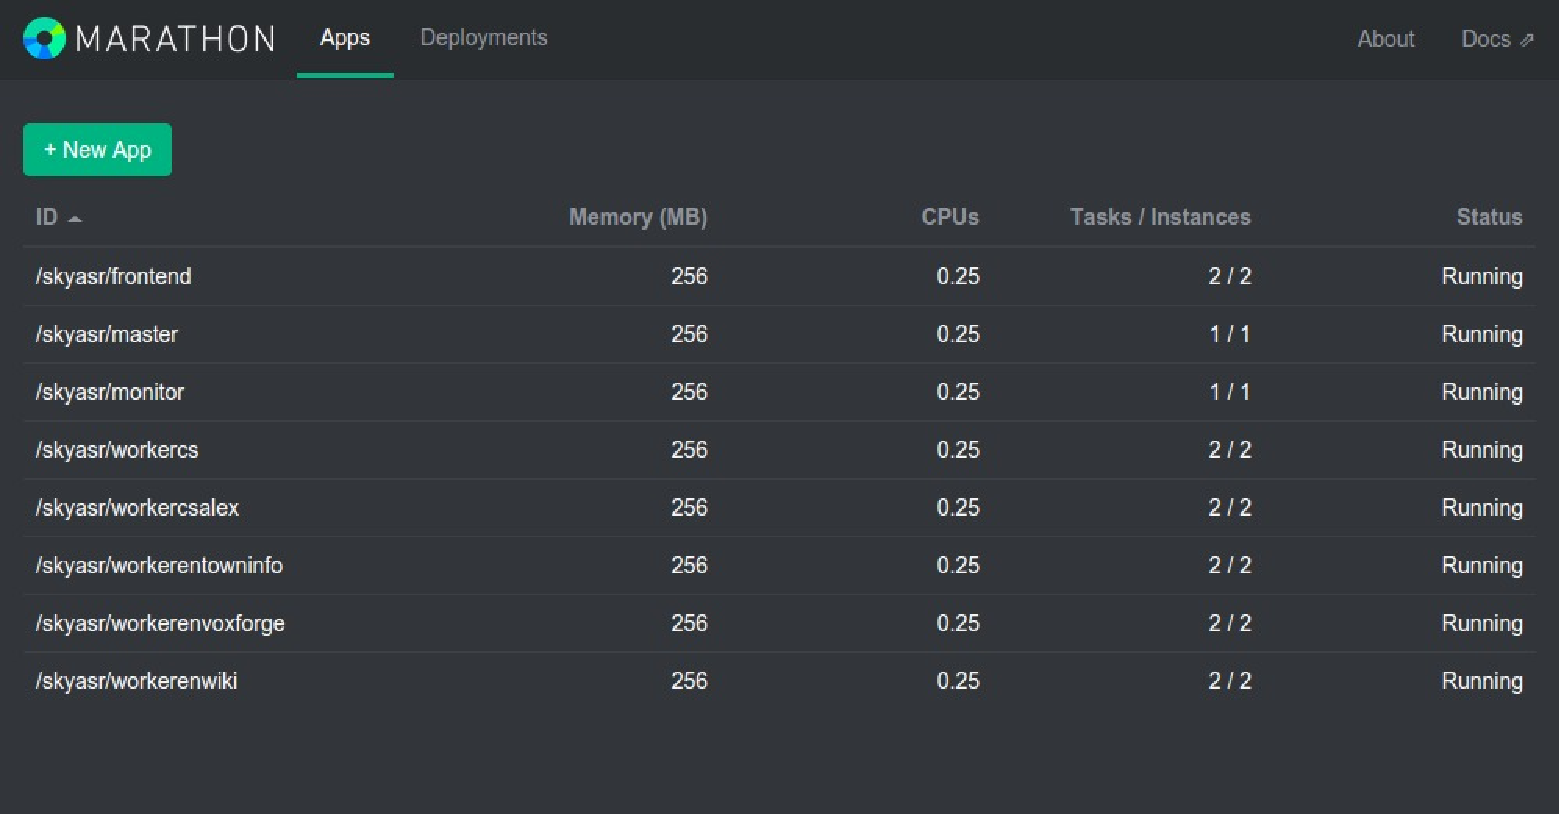
\includegraphics[width=0.95\textwidth]{./img/marathon.pdf}

  \caption{
    A screenshot of a Marathon web interface with a running CloudASR platform.
  }
  \label{fig:marathon}
\end{figure}

Since the traffic of CloudASR platform can be very large,
  it is not possible to process all HTTP requests by one application server.
Therefore, CloudASR platform uses \textbf{HAProxy}\footnote{\url{http://www.haproxy.org/}} load-balancer to distribute workload between application servers,
  but any other load-balancers can also be used with appropriate setup.



\section{Continuous Integration \& Delivery}
Several practises were obeyed during the development,
  namely Continuous Integration and Continuous Delivery.
For this a platform which consisted of \textbf{Jenkins-CI}\footnote{\url{https://jenkins-ci.org/}} and \textbf{Docker Registry}\footnote{\url{https://github.com/docker/docker-registry}} was deployed.

The most important tool for Continuous Integration \& Delivery of CloudASR is Jenkins-CI.
Its task is to watch CloudASR git repository
  and whenever a new code is pushed into this repository it schedules a new build of the platform.
During this build, the most recent code is pulled from the repository and then the new docker images are built.
After that tests are run to check that the new code did not break anything.
Finally, successfully built images are tagged with current build number and pushed to the Docker Registry.


Docker Registry is a repository of Docker images.
Even though, there are several Docker Registry providers\footnote{\url{https://hub.docker.com/}, \url{https://quay.io/}},
  which are free for open-source projects,
  CloudASR uses its own free Docker Registry in order to be able to use also proprietary software that cannot be shared with public.


\section{Backend}
The main programming language used for backend development is \textbf{Python}\footnote{\url{https://www.python.org/}}.
The web interface is built on top of \textbf{Flask}\footnote{\url{http://flask.pocoo.org/}} microframework
  and it uses \textbf{Gunicorn}\footnote{\url{http://gunicorn.org/}} for production deployment.
\textbf{MySQL}\footnote{\url{https://www.mysql.com/}} is used as a database,
  but any other SQL database can be used instead,
  because the database is accessed  through \textbf{SQLAlchemy}\footnote{\url{http://www.sqlalchemy.org/}}.

The CloudASR architecture consists of several nodes which need to communicate between each other.
CloudASR uses \textbf{ZeroMQ}\footnote{\url{http://zeromq.org/}} for this communication
  because of its simple design, high performance and support for every modern language.
With ZeroMQ,
  it is possible to create many messaging patterns,
  but CloudASR uses only two: request-reply and push-pull.
In the request-reply messaging pattern a sender sends a message and then waits for a reply,
  after that another sender can send next message and wait for a reply.
On the other hand, in the push-pull messaging pattern senders just send messages and do not wait for replies.


In order to be able to send complex messages via ZeroMQ sockets, messages have to be serialized.
CloudASR uses \textbf{Google Protocol Buffers}\footnote{\url{https://developers.google.com/protocol-buffers/}},
  because they have support in many languages,
  allow specification of various message types (See Figure~\ref{fig:protobuf} for example)
  and serialize messages in very compact way
  (See Table~\ref{fig:protobuf-benchmark} for a comparison of different serializations).

\begin{figure}[h]
  \verbatiminput{snippets/protobuf.proto}

  \caption{
    An example of Google Protocol Buffer message specification with three fields.
    Fields address and model are just strings and the status is an enum with four possible values.
  }
  \label{fig:protobuf}
\end{figure}

\begin{table}[h]
  \begin{tabular}{rrl}
  \textbf{raw file size} & 56146 & \\
  \cline{1-3}
  \textbf{bytes\_protobuf} & 56118 & 0.999x \\
  \textbf{base64} & 74872 & 1.333x \\
  \textbf{json\_array} & 158590 & 2.824x \\
  \end{tabular}

  \caption{
    The table shows comparison of different serialization used to serialize a wave file into a message for the CloudASR online mode.
    As can be seen from the results Google Protocol Buffers achieved the best result.
  }
  \label{fig:protobuf-benchmark}
\end{table}

CloudASR uses \textbf{Pykaldi} \cite{platek2014free} as a Python wrapper for the \textbf{Kaldi speech recognition toolkit} \cite{povey2011kaldi}.
Because CloudASR should be able to process very long recordings, possibly infinite,
  with limited computational resources,
  it is necessary to split the recordings into smaller chunks.
For that purpose CloudASR uses voice activity detector implemented in \textbf{Theano} \cite{bergstra2010theano} to detect silences in a speech.


\section{Frontend}
The frontend uses several well-known open-source libraries, namely,
  \textbf{Twitter Bootstrap}\footnote{\url{http://getbootstrap.com/2.3.2/}} for CSS styling of the web,
  \textbf{jQuery}\footnote{\url{https://jquery.com/}}
  and \textbf{Angular.js}\footnote{\url{https://angularjs.org/}} for interactive elements on the web.

\begin{figure}[h]
  \centering
  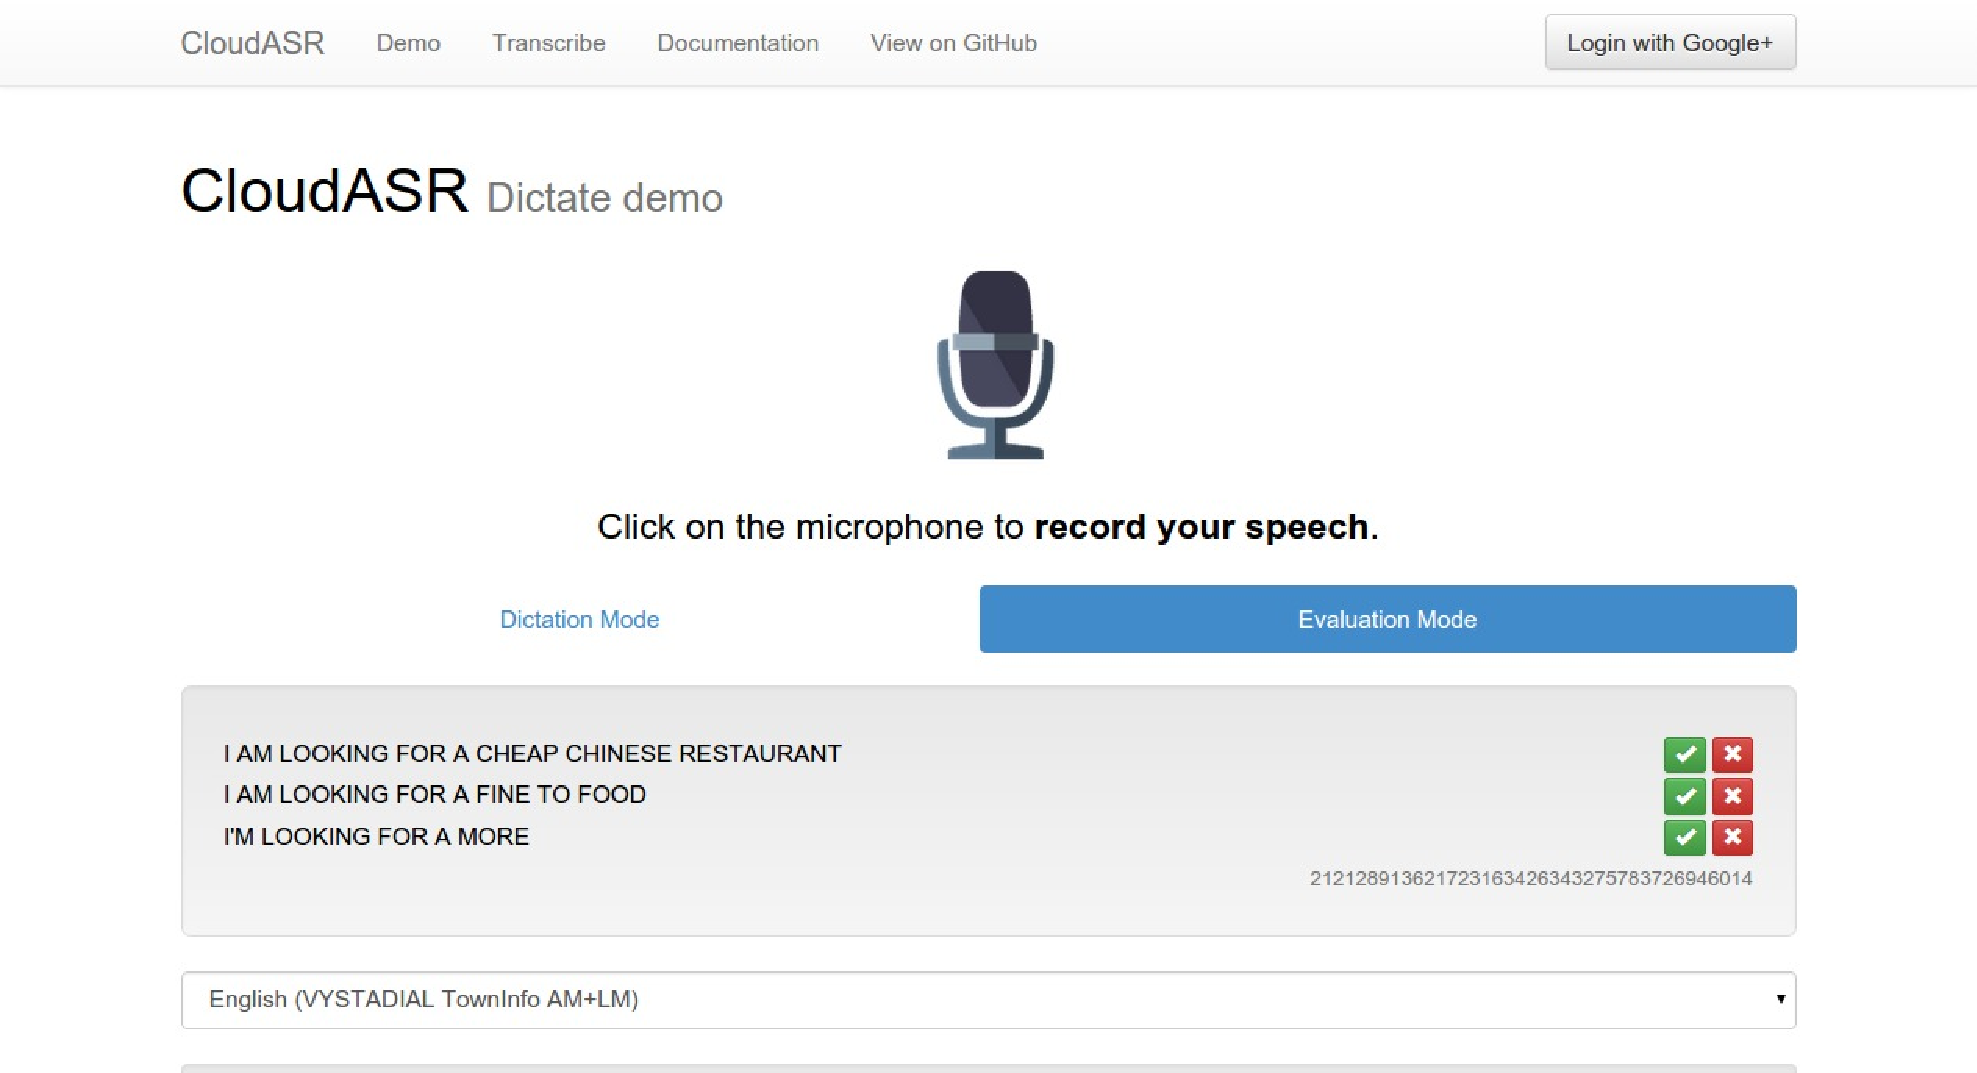
\includegraphics[width=0.95\textwidth]{./img/demo.pdf}

  \caption{Screen of the Web Demo.}
  \label{fig:demo}
\end{figure}

Modern web browsers support \textbf{WebAudio API}\footnote{\url{http://webaudio.github.io/web-audio-api/}},
  which is a high-level JavaScript API for processing and synthesizing audio in web applications.
One of the things that can be done with this API is audio recording.
Thus, it is possible to create a web demo for the CloudASR online mode.
The demo is based on \textbf{Recorder.js}\footnote{\url{https://github.com/mattdiamond/Recorderjs}} library,
  which can record output of WebAudio API and return it as a PCM chunks.

The next step is to send these chunks to the API.
Because the demo demonstrates the online speech recognition mode,
  it is not possible to wait for the whole recording to be recorded and then send it to the API via HTTP POST request.
Thus, CloudASR uses \textbf{Socket.IO}\footnote{\url{http://socket.io/}} to send stream of chunks to the API
  and to receive stream of results from the API.

\chapter{Solution}
\blindtext

\section{Architecture}
\blindtext

\subsection{Frontend}
\blindtext

\subsection{Master}
\blindtext

\subsection{Worker}
\blindtext

\subsection{Annotation Interface}
\blindtext


\section{Request Workflow}
\blindtext

\subsection{Batch Recognition}
\blindtext

\subsection{Online Recognition}
\blindtext


\section{Deployment}
\blindtext

\subsection{Single-Host Deployment}
\blindtext

\subsection{Multi-Host Deployment}
\blindtext

\subsection{Contiunous Integration \& Countinuous Delivery}
\blindtext


\section{Hosting Various Models}
\blindtext

\subsection{Worker Deployment}
\blindtext
\blindtext

\subsection{Phonexia's Models}
\blindtext

\subsection{Kaldi Models}
\blindtext

\chapter{Evaluation}\label{chapter:evaluation}
In order to show that the CloudASR platform is ready for the production usage
  several benchmarks were made.
First, real time factor (RTF) of the batch speech recognition mode was measured and compared with Google Speech API.
Second, latency of the online speech recognition mode was measured.
Finally, number of parallel requests for batch speech recognition mode was measured.
These benchmarks will be described in the following section.


\section{RTF of Batch Speech Recognition}
In the first benchmark RTF of CloudASR batch mode was compared with RTF of Google Speech API
  using test set from the Czech Public Transportation Information Domain \cite{korvas2014vystadial}.
WER and RTF of both APIs were measured with following results:
Google Speech API had 60\% WER and RTF 0.3 whereas
  CloudASR had 22\% WER and RTF 0.22.
Request times of both APIs are displayed in Figure~\ref{fig:batch-benchmark}.

This benchmark shows that RTF of CloudASR batch mode is better than RTF of Google Speech API.
Moreover, the benchmark shows that the CloudASR platform can achieve better accuracy than Google Speech API on limitted domains
  if the used decoding graphs are customized for that domains.

\begin{figure}[h]
  \centering
  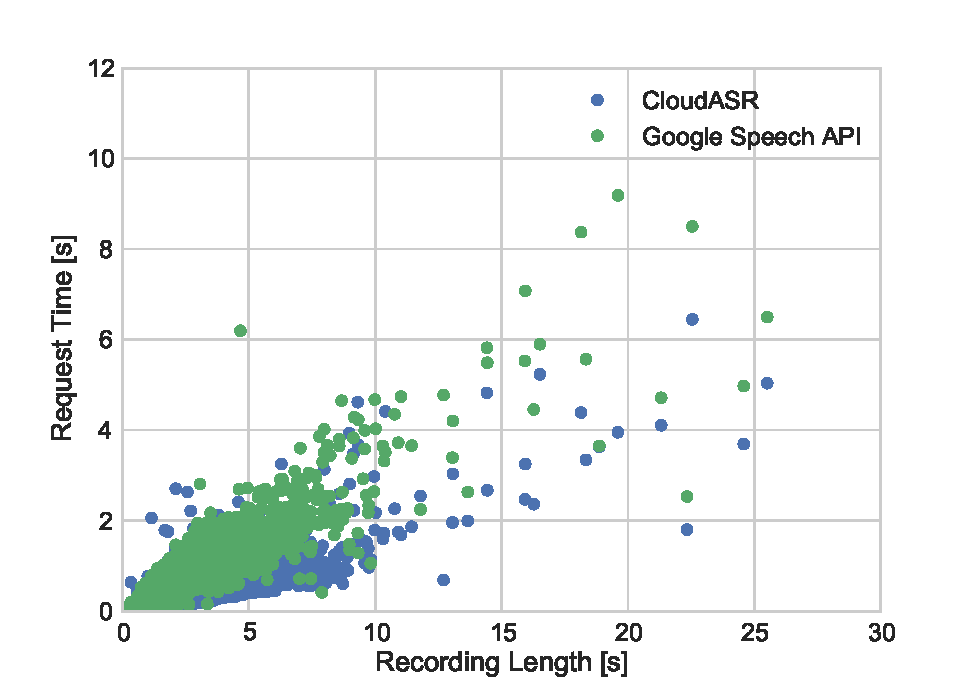
\includegraphics[width=0.75\textwidth]{./img/batch.pdf}

  \caption{
    Batch recognition benchmark.
  }
  \label{fig:batch-benchmark}
\end{figure}



\section{Latency of Online Speech Recognition}
In the second benchmark latency of CloudASR online mode was measured.
Since the low latency is crucial for successfull usage of speech recognition in dialogue systems
  and there are not so many webservice that provide online speech recognition mode
  support for online speech recognition mode can be seen as a key feature of the CloudASR platform.
The reason why the online speech recognition mode is better suited for dialogue systems is
  that it is not neccessary to wait for the whole recording to be recorded
  and instead it is possible to get the interim results while the speech is recorded.
Thus, dialogue systems can react quickly.
Figure~\ref{fig:online-benchmark} shows comparison of the deelay between utterance end and the availability of the recognition results for CloudASR online and batch mode.

\TODO{add conclusion}

\begin{figure}[h]
  \centering
  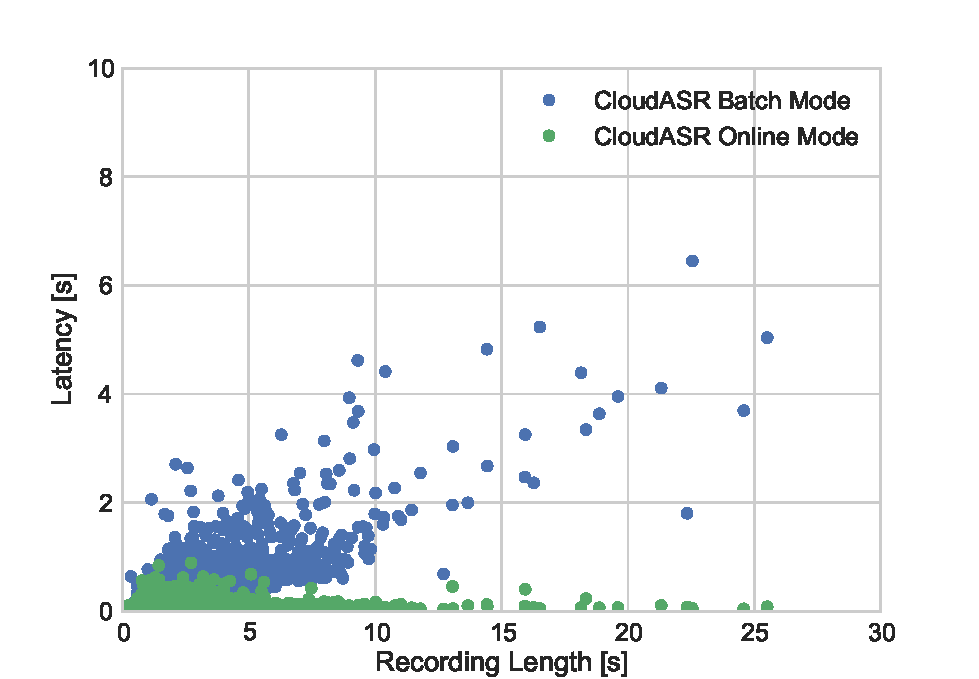
\includegraphics[width=0.75\textwidth]{./img/online.pdf}

  \caption{
    A latency comparison for CloudASR online and batch mode.
  }
  \label{fig:online-benchmark}
\end{figure}


\section{Parallel Requests Benchmark}
Since the main bottleneck of the CloudASR platform is a number of running workers
  workers with dummy asr engine (described in Figure~\ref{fig:dummyasr})
  that would enable to test how many parallel requests can CloudASR handle were used.
As a result, 1000 dummy workers could run on a Mesos cluster with 5 slaves (4CPU, 16GB RAM).
Also, HAProxy load-balancer, which spread workload accross 5 frontend containers, was deployed.

Then several benchmarks were run to show how RTF of the batch recognition mode changes with different number of parallel requests.
The platform was tested with a different number of parallel requests (50, 250, 500, 750 and 1000)
  and with files with different lengths (5s, 10s, 20s, 30s, 40s, 50s and 60s).
Results are summarized on Figure~\ref{fig:parallel-benchmark}.

Results show that CloudASR platform adds just a very little overhead compared to the raw dummy worker.
Moreover, results shows that the platform is able to handle much more parallel requests with appropriate number of workers.

\IDEA{Network capacity, similarity to online recognition}

\begin{figure}[h]
  \centering
  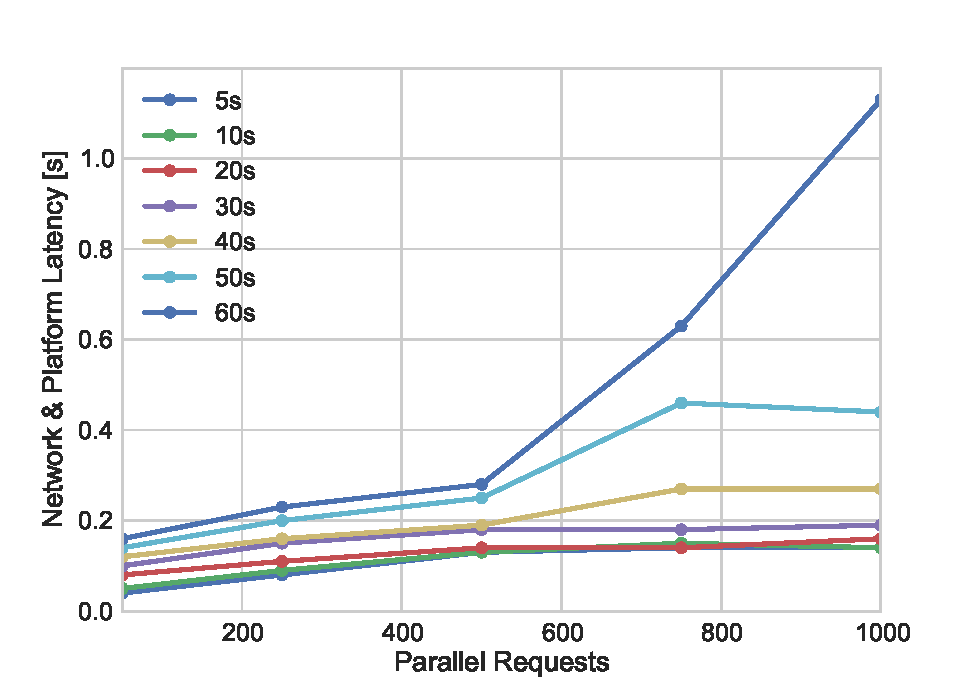
\includegraphics[width=0.75\textwidth]{./img/parallel.pdf}

  \caption{
    The graph shows platform \& network latency for recordings with various lengths
      given the number of parallel requests.
  }
  \label{fig:parallel-benchmark}
\end{figure}


% Ukázka použití některých konstrukcí LateXu (odkomentujte, chcete-li)
% %%% Ukázka použití některých konstrukcí LaTeXu

\subsection{Ukázka \LaTeX{}u}
\label{ssec:ukazka}

This short subsection serves as an~example of basic \LaTeX{} constructs,
which can be useful for writing a~thesis.

Let us start with lists:

\begin{itemize}
\item The logo of Matfyz is displayed in figure~\ref{fig:mff}.
\item This is subsection~\ref{ssec:ukazka}.
\item Citing literature~\cite{lamport94}.
\end{itemize}

Different kinds of dashes:
red-black (short),
pages 16--22 (middle),
$45-44$ (minus),
and this is --- as you could have expected --- a~sentence-level dash,
which is the longest.
(Note that we have follwed \verb|a| by a~tilde instead of a~space
to avoid line breaks at that place.)

\newtheorem{theorem}{Theorem}
\newtheorem*{define}{Definition}	% Definice nečíslujeme, proto "*"

\begin{define}
A~{\sl Tree} is a connected graph with no cycles.
\end{define}

\begin{theorem}
This theorem is false.
\end{theorem}

\begin{proof}
False theorems do not have proofs.
\end{proof}

\begin{figure}
	\centering
	
\includegraphics[width=30mm]{../img/logo.eps}
	\caption{Logo of MFF UK}
	\label{fig:mff}
\end{figure}


\chapter*{Conclusion}
\addcontentsline{toc}{chapter}{Conclusion}

Goals of this thesis were to develop a cloud platform for ASR, CloudASR,
  and an annotation interface for annotating speech data.
These goals were successfully accomplished and in several aspects even surpassed
  - in addition to original requirement to create batch recognition mode,
  online speech recognition mode was implemented.
In the following sections all achievements are summarized and
  at the end ideas for future work are proposed.

\section*{Cloud platform for ASR}
The first goal of this thesis was to develop a cloud platform for ASR, CloudASR,
  that would provide API for batch speech recognition mode of the submitted wave files.
This API is similar to Google Speech API,
  which enables users to switch to CloudASR seamlessly.
In addition to that CloudASR provides an API for online speech recognition mode.
The CloudASR comes with a web demo,
  where the users can try out the online speech recognition mode with various languages.
Furthermore, the platform is scalable, customizable and easily deployable.


In terms of scalability,
  the platform is able to run both on single-machine and multi-machine setup
  and it allows to scale number of running workers according to users' needs.
Additionally, the platform can run several API instances and load-balance between them.
The benchmarks show that the platform is able to handle more than 1000 parallel requests
  given enough computational resources.

The platform can handle requests for various languages at the same time.
Moreover, users can create workers for new languages using Pykaldi
  or they can even create workers for an arbitrary ASR systems
  if they provide a Python wrapper for that system.

Finally, CloudASR is easily deployable.
It uses Docker for creating and running application containers.
Therefore, users have to install only Docker for a single machine setup
  and a Mesos cluster for a multi machine setup.
Then it is possible to run the CloudASR platform with just one command.


\section*{Annotation interface}
The second goal of this thesis was to create an annotation interface for annotating submitted recordings.
Its responsibility is to collect and store obtained recordings together with their transcriptions.
Then users can rate transcriptions of the recordings
  or they can add their own transcriptions
  if they think that none is correct.
The annotation interface allows administrators to choose golden transcription from several manual transcriptions
  that were obtained for the recording.
Additionally CloudASR also supports addition of manual transcriptions via external job at CrowdFlower.

\section*{Future work}
\begin{itemize}
  \item
    Since manual transcription of recordings is expensive
      it would be good to make users transcribe only parts of the recordings
      in which ASR system wasn't confident enough \cite{sperber2014fly}.
    This idea could be used for both user transcription and CrowdFlower transcription.

  \item
    With manually transcribed recordings from CloudASR platform
      it is possible to continuously improve accuracy of the underlying ASR system
      by adapting the language model to the type of language that the users of the CloudASR really use.
    Thus CloudASR could provide an option to automatically update language model
      when a certain amount of new transcribed recordings was collected.

  \item
    Because running CloudASR platform is expensive in terms of costs for a server hosting,
      it would be good to optimize usage of individual workers
      so that spare workers are shut down when there is no need for them
      and new workers are started when the traffic arise.
    This can be achieved either by providing feedback control based systems \cite{janert2013feedback}
      or by using machine learning techniques \cite{gong2010press}.

  \item
    As CloudASR platform provides API for speech recognition,
      it could also be used for another speech related tasks like Language Identification, Speaker Identification, Voice Activity Detection, etc.

\end{itemize}




%%% Seznam použité literatury
%%% Seznam použité literatury je zpracován podle platných standardů. Povinnou citační
%%% normou pro diplomovou práci je ISO 690. Jména časopisů lze uvádět zkráceně, ale jen
%%% v kodifikované podobě. Všechny použité zdroje a prameny musí být řádně citovány.

\phantomsection
\addcontentsline{toc}{chapter}{\bibname}
\nocite{*}
\bibliography{citations}{}
\bibliographystyle{amsplain}

%\bibitem{lamport94}
%  {\sc Lamport,} Leslie.
%  \emph{\LaTeX: A Document Preparation System}.
%  2. vydání.
%  Massachusetts: Addison Wesley, 1994.
%  ISBN 0-201-52983-1.



%%% Tabulky v diplomové práci, existují-li.
\chapwithtoc{List of Tables}

%%% Použité zkratky v diplomové práci, existují-li, včetně jejich vysvětlení.
\chapwithtoc{List of Abbreviations}

%%% Přílohy k diplomové práci, existují-li (různé dodatky jako výpisy programů,
%%% diagramy apod.). Každá příloha musí být alespoň jednou odkazována z vlastního
%%% textu práce. Přílohy se číslují.
\chapwithtoc{Attachments}

\openright
\end{document}
